\subsection{Vì sao cần mô phỏng, và mô phỏng cái gì}
Câu hỏi hợp lý đầu tiên là: trên máy tính không có không khí, không có gió, không có cồn --- vậy những con số so sánh ba thuật toán ở đâu ra?

Câu trả lời ngắn: \textbf{nhóm không mô phỏng không khí. Nhóm mô phỏng \textit{hệ quả} của không khí lên chất khí, bằng một tập quy tắc.} ``Gió'' trong chương trình không phải là không khí đang chuyển động; nó là \textbf{một vectơ cộng vào toạ độ của mỗi đám khí sau mỗi bước thời gian}. Và đối với chất khí đang trôi, gió thật cũng chỉ làm đúng chừng ấy việc.

Mô phỏng phục vụ ba mục đích cụ thể trong đề tài: kiểm tra logic ba thuật toán trước khi có phần cứng; dò tham số (ngưỡng, bước đi, biên độ cast) với chi phí gần bằng không; và tạo ra một bộ số liệu so sánh \textbf{có kiểm soát hoàn toàn}, trong đó mọi yếu tố ngoài thuật toán đều được giữ giống hệt nhau.


\subsection{Ba mô hình ghép lại}
\begin{figure}[!p]
  \centering
  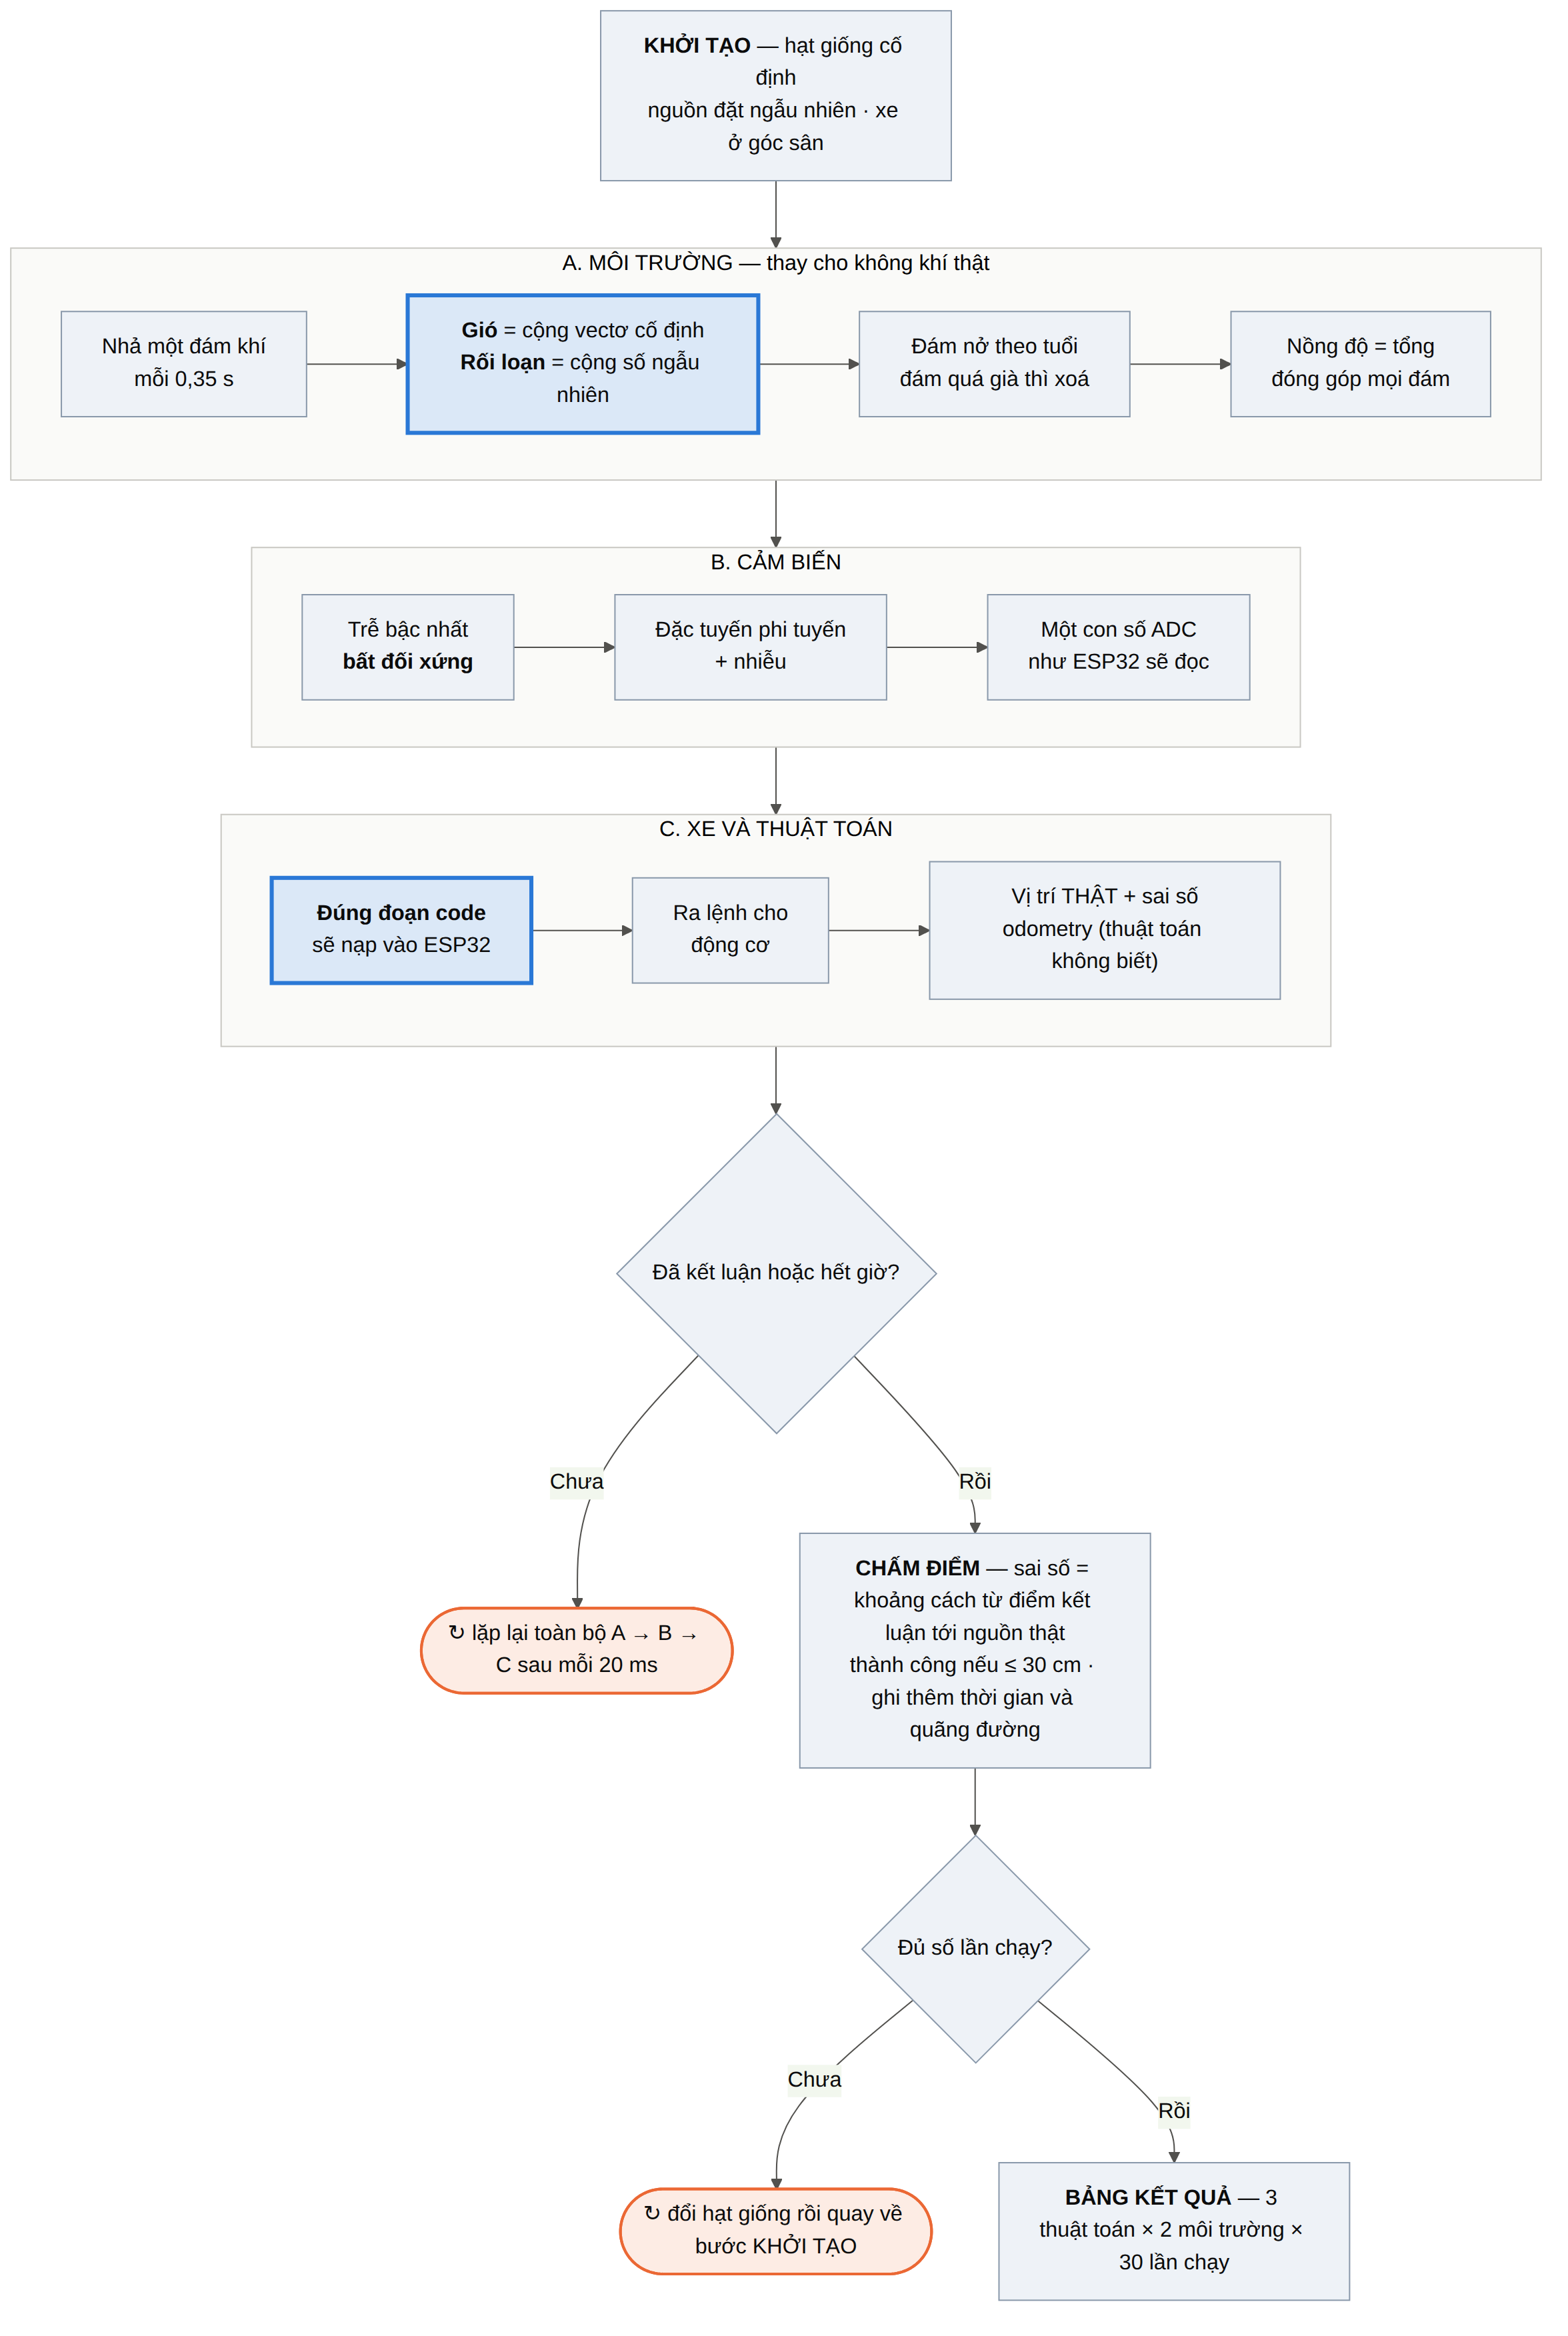
\includegraphics[width=0.885\textwidth]{pic/8_vong_lap_mo_phong.png}
  \caption{Vòng lặp mô phỏng. Thuật toán chỉ nhìn thấy vị trí mà xe \textit{tưởng} là mình đang đứng; việc chấm điểm dùng vị trí thật.}
\end{figure}

\subsubsection{Mô hình môi trường}
Hình 5.1 trình bày toàn bộ vòng lặp mô phỏng và ba mô hình hợp thành. Với \textbf{môi trường khuếch tán thuần} (không quạt), trường nồng độ được mô tả bằng một hàm giảm đơn điệu, trơn và không kỳ dị tại tâm:

\[ C(r) = \frac{r_0^{2}}{r_0^{2}+r^{2}} \qquad\text{với } r_0 = 25~\text{cm} \]
Đây đúng là điều kiện lý tưởng mà bám gradient cần.

Với \textbf{môi trường phát tán đứt quãng} (có quạt), nhóm dùng \textbf{mô hình puff} --- mô hình ``đám khí'' --- hoạt động theo năm bước:

\begin{enumerate}[leftmargin=1.6em,itemsep=0.15em,topsep=0.3em]
  \item Nguồn phát nhả ra một \textbf{đám khí nhỏ} sau mỗi 0,35 giây. Mỗi đám là một chấm có toạ độ, có tuổi và mang một lượng chất nhất định.
  \item Sau mỗi bước thời gian 20 ms, \textbf{mọi đám đều dịch chuyển}. Phần dịch chuyển gồm hai thành phần cộng lại: một \textbf{vectơ cố định} --- đó là gió trung bình, 25 cm/s --- và một \textbf{số ngẫu nhiên} --- đó là rối loạn, biên độ 14 cm/s.
  \item Mỗi đám \textbf{nở rộng theo tuổi}: bình phương bán kính tăng tuyến tính theo thời gian, với tốc độ 70 cm$^{2}$/s. Đây chính là dạng toán học của khuếch tán.
  \item Đám nào quá già (trên 22 giây) thì bị xoá, để chương trình không phình vô hạn.
  \item \textbf{Nồng độ tại một điểm bất kỳ bằng tổng đóng góp của tất cả các đám còn sống}, mỗi đám đóng góp theo một hàm Gauss quanh tâm của nó.
\end{enumerate}
Đây là dạng rút gọn của mô hình filament do Farrell và cộng sự công bố năm 2002 trên \textit{Environmental Fluid Mechanics} [2] --- mô hình tiêu chuẩn để tạo cấu trúc đứt quãng của luồng mùi trong nghiên cứu robot khứu giác. Cùng họ mô hình đó được dùng trong bộ mô phỏng GADEN công bố trên \textit{Sensors} năm 2017 [4].

\begin{ghichu}
Một chi tiết kỹ thuật nhỏ nhưng quyết định tính đúng đắn: số ngẫu nhiên biểu diễn rối loạn được nhân với \textbf{căn bậc hai của bước thời gian}, chứ không nhân với bước thời gian. Đó là quy luật đúng của một bước đi ngẫu nhiên. Nếu làm sai, kết quả mô phỏng sẽ \textbf{phụ thuộc vào việc chọn bước thời gian bao nhiêu} --- và khi đó mọi con số đều mất ý nghĩa.
\end{ghichu}

\subsubsection{Mô hình cảm biến}
Nồng độ tính được ở trên là một đại lượng toán học, chưa phải cái mà vi điều khiển đọc được. Nó được đưa qua một mô hình cảm biến ba tầng:

\begin{itemize}[leftmargin=1.4em,itemsep=0.15em,topsep=0.3em]
  \item Một khâu \textbf{trễ bậc nhất bất đối xứng}: hằng số thời gian khi lên là \textbf{2,5 giây}, khi xuống là \textbf{8 giây} --- đúng đặc tính lên nhanh xuống chậm của cảm biến oxit kim loại đã mô tả ở mục 2.3. Đây là chi tiết quan trọng nhất của mô hình, vì chính nó buộc phải có quy trình ``dừng ngửi'' và cơ chế quay lại điểm tốt nhất.
  \item Một \textbf{đặc tuyến phi tuyến dưới tuyến tính} (số mũ 0,75), mô phỏng việc cảm biến bão hoà dần ở nồng độ cao.
  \item Một lượng \textbf{nhiễu ngẫu nhiên} với độ lệch chuẩn 4 đếm ADC.
\end{itemize}
Đầu ra là một con số ADC nằm trong cùng dải giá trị với con số thật mà ESP32 sẽ đọc.


\subsubsection{Mô hình xe và sai số dead reckoning}
Mô hình xe gồm toạ độ, hướng, tốc độ chạy 18 cm/s và tốc độ quay 90 $^\circ$/s. Chi tiết quan trọng nhất về mặt trung thực: chương trình giữ \textbf{hai vị trí khác nhau} cho chiếc xe --- \textbf{vị trí thật} và \textbf{vị trí mà xe tưởng là mình đang đứng}. Hai vị trí này lệch dần theo thời gian vì ba nguồn sai số: sai số tỉ lệ quãng đường $\pm$1,5 \%, trôi con quay $\pm$0,06 $^\circ$/s, và sai số $\pm$1,2$^\circ$ cho mỗi lần quay.

\textbf{Thuật toán chỉ được nhìn thấy vị trí mà xe tưởng.} Việc chấm điểm thì dùng vị trí thật. Nhờ vậy con số sai số định vị trong bảng kết quả không bị đẹp giả tạo.

\begin{table}[!htbp]
  \centering
  \caption{Tham số của mô hình mô phỏng}
  \small
  \renewcommand{\arraystretch}{1.25}
  \begin{tabular}{>{\raggedright\arraybackslash}p{0.3793\textwidth}>{\raggedright\arraybackslash}p{0.1806\textwidth}>{\raggedright\arraybackslash}p{0.3432\textwidth}}
    \toprule
    \textbf{Tham số} & \textbf{Giá trị} & \textbf{Ghi chú} \\
    \midrule
    Bước thời gian mô phỏng & 20 ms & Trùng với chu kỳ vòng điều khiển thật \\
    Bán kính đặc trưng (khuếch tán) & 25 cm &  \\
    Tốc độ gió (đứt quãng) & 25 cm/s &  \\
    Chu kỳ nhả đám khí & 0,35 s &  \\
    Bán kính đám khí lúc mới nhả & 5 cm &  \\
    Tốc độ nở của đám khí & 70 cm$^{2}$/s & R$^{2}$ tăng tuyến tính theo thời gian \\
    Biên độ rối loạn ngang & 14 cm/s & Bước đi ngẫu nhiên \\
    Tuổi tối đa của một đám khí & 22 s &  \\
    Hằng số thời gian cảm biến, chiều lên & 2,5 s &  \\
    Hằng số thời gian cảm biến, chiều xuống & 8 s & Bất đối xứng --- đặc tính MOX \\
    Nhiễu ADC & 4 đếm (độ lệch chuẩn) &  \\
    Tốc độ chạy của xe & 18 cm/s &  \\
    Tốc độ quay của xe & 90 $^\circ$/s &  \\
    Sai số tỉ lệ quãng đường & $\pm$1,5 \% &  \\
    Trôi con quay hồi chuyển & $\pm$0,06 $^\circ$/s &  \\
    Sai số mỗi lần quay & $\pm$1,2$^\circ$ &  \\
    \bottomrule
  \end{tabular}
\end{table}
\begin{ghichu}
\textbf{Giới hạn phải nói rõ:} mọi tham số trong Bảng 5.1 là \textbf{giả định của nhóm}. Chúng được chọn để tạo ra một trường nồng độ có dạng hình học và động học hợp lý, đủ để so sánh \textbf{hành vi} của ba thuật toán. Chúng \textbf{không phải} số liệu đo được từ thực địa. Vì vậy kết quả mô phỏng được trình bày ở một chương riêng và không được trộn lẫn với số liệu thực nghiệm.
\end{ghichu}

\subsection{Vòng lặp mô phỏng}
Mỗi 20 mili-giây, chương trình thực hiện đúng chuỗi việc sau: cập nhật vị trí tất cả các đám khí $\rightarrow$ tính nồng độ tại đầu cảm biến theo \textbf{vị trí thật} của xe $\rightarrow$ cho qua mô hình cảm biến để ra con số ADC $\rightarrow$ \textbf{đưa con số đó cho thuật toán} $\rightarrow$ thuật toán ra lệnh cho động cơ $\rightarrow$ cập nhật vị trí xe và cộng thêm sai số odometry. Rồi lặp lại.

Điểm mấu chốt của toàn bộ chương này: \textbf{đoạn mã thuật toán chạy trong mô phỏng chính là đoạn mã sẽ nạp vào ESP32.} Không phải bản viết lại, không phải bản mô tả. Nhờ kiến trúc trình bày ở mục 4.1, phần thuật toán chỉ gọi những lệnh trừu tượng như ``đi tới'', ``quay'', ``đọc khí''; khi chạy trên xe, các lệnh đó nối vào phần cứng thật, khi chạy trên máy tính chúng nối vào mô hình. Nghĩa là \textbf{không tồn tại rủi ro ``bản mô phỏng khác bản thật''}: nếu thuật toán có lỗi logic, mô phỏng sẽ bộc lộ đúng lỗi đó.


\subsection{Thiết kế thí nghiệm và tiêu chí chấm điểm}
\begin{table}[!htbp]
  \centering
  \caption{Thiết kế thí nghiệm mô phỏng}
  \small
  \renewcommand{\arraystretch}{1.25}
  \begin{tabular}{>{\raggedright\arraybackslash}p{0.3158\textwidth}>{\raggedright\arraybackslash}p{0.6130\textwidth}}
    \toprule
    \textbf{Yếu tố} & \textbf{Cấu hình} \\
    \midrule
    Biến độc lập 1 --- thuật toán & 3 mức: quét toàn bộ $\cdot$ bám gradient $\cdot$ surge-casting \\
    Biến độc lập 2 --- môi trường & 2 mức: khuếch tán thuần $\cdot$ phát tán đứt quãng \\
    Số lần lặp mỗi tổ hợp & N = 30 \\
    Tổng số lần chạy & 3 $\times$ 2 $\times$ 30 = 180 \\
    Vị trí nguồn & Ngẫu nhiên trong vùng x $\in$ [50 \%, 90 \%] và y $\in$ [20 \%, 80 \%] của sân \\
    Ghép cặp & \textbf{Cùng một hạt giống cho cả ba thuật toán} --- ba thuật toán gặp đúng cùng một vị trí nguồn \\
    Biến phụ thuộc 1 & Thành công / thất bại (nhị phân) \\
    Biến phụ thuộc 2 & Thời gian định vị (giây) \\
    Biến phụ thuộc 3 & Sai số định vị (cm) \\
    Biến phụ thuộc 4 & Quãng đường đã đi (m) \\
    Thời gian tối đa mỗi lần chạy & 480 giây \\
    \bottomrule
  \end{tabular}
\end{table}
Bảng 5.2 tóm tắt toàn bộ thiết kế thí nghiệm. \textbf{Tiêu chí thành công.} Khi thuật toán tuyên bố ``đây là nguồn'', chương trình đo khoảng cách từ vị trí thật của đầu dò tới vị trí thật của nguồn. Nếu khoảng cách đó \textbf{không quá 30 cm} thì tính là thành công. Ngưỡng 30 cm được chọn tương ứng với hơn một ô lưới một chút --- đủ chặt để loại các kết luận sai rõ ràng, đủ rộng để không phạt robot vì sai số dead reckoning tích luỹ.

\textbf{Tính lặp lại.} Mọi số ngẫu nhiên đều sinh từ một hạt giống cố định, nên mỗi lần chạy trong bảng kết quả đều \textbf{tái lập được tới từng bước}. Việc dùng chung hạt giống giữa ba thuật toán bảo đảm chúng gặp đúng cùng một bài toán, loại bỏ hoàn toàn ảnh hưởng của việc ``nguồn đặt ở chỗ dễ hay khó''.


\subsection{Mô phỏng này chứng minh được gì và không chứng minh được gì}
Đây là điểm nhóm muốn phát biểu thật rõ ràng, vì nó quyết định cách đọc toàn bộ Chương 6.

\textbf{Mô phỏng chứng minh được:} ba thuật toán, khi chạy trên \textbf{cùng một trường khí, cùng một mô hình cảm biến, cùng một bộ hạt giống và cùng một cách chấm điểm}, cho ra thứ hạng như thế nào. Vì mọi yếu tố khác đều giống hệt nhau, phần chênh lệch quan sát được chỉ có thể quy cho bản thân thuật toán.

\textbf{Mô phỏng không chứng minh được:} các con số tuyệt đối. Nhóm \textbf{không} khẳng định rằng ngoài thực tế surge-casting sẽ thành công 57 \%. Bộ tham số của mô hình được chọn để tạo ra một trường có động học hợp lý, không phải đo từ thực địa.

\begin{ghichu}
\textbf{Phản biện đã lường trước:} ``Các em tự chọn tham số thì có phải cứ chỉnh tham số là ra kết quả mình muốn không?'' Cách phòng vệ đúng cho câu hỏi này là \textbf{phân tích độ nhạy}: thay đổi tốc độ gió, chu kỳ nhả khí và hằng số thời gian cảm biến trong khoảng $\pm$50 \%, rồi kiểm tra xem \textbf{thứ hạng ba thuật toán có đảo không}. Nếu thứ hạng giữ nguyên trên cả dải tham số thì kết luận không phụ thuộc vào bộ tham số cụ thể. Nhóm ghi nhận đây là phần \textbf{chưa hoàn thành}, và xếp nó vào hướng phát triển ở mục 7.3.
\end{ghichu}
